\documentclass[12pt,a4paper]{article}
\usepackage[ngerman]{babel}
\usepackage[utf8]{inputenc}
\usepackage{amsmath}
\usepackage{amsfonts}
\usepackage{amssymb}
\usepackage{graphicx}
\usepackage{fancyhdr}
\usepackage{tabularx}
\usepackage{geometry}
\usepackage{setspace}
\usepackage[right]{eurosym}
\usepackage[printonlyused]{acronym}
\usepackage{subfig}
\usepackage{floatflt}
\usepackage[usenames,dvipsnames]{color}
\usepackage{colortbl}
\usepackage{paralist}
\usepackage{array}
\usepackage{titlesec}
\usepackage{parskip}
\usepackage[right]{eurosym}
\usepackage{picins}
\usepackage[subfigure,titles]{tocloft}
\usepackage[pdfpagelabels=true]{hyperref}

\usepackage{listings}
\lstset{basicstyle=\footnotesize, captionpos=b, breaklines=true, showstringspaces=false, tabsize=2, frame=lines, numbers=left, numberstyle=\tiny, xleftmargin=2em, framexleftmargin=2em}
\makeatletter
\def\l@lstlisting#1#2{\@dottedtocline{1}{0em}{1em}{\hspace{1,5em} Lst. #1}{#2}}
\makeatother

\geometry{a4paper, top=27mm, left=20mm, right=20mm, bottom=35mm, headsep=10mm, footskip=12mm}


\hypersetup{unicode=false, pdftoolbar=true, pdfmenubar=true, pdffitwindow=false, pdfstartview={FitH},
	pdftitle={HSP: Reinforcement Learning (WS \the\year)},
	pdfauthor={Dr.\ Carsten Kern},
	pdfsubject={Projektbericht},
	pdfcreator={\LaTeX\ with package \flqq hyperref\frqq},
	pdfproducer={pdfTeX \the\pdftexversion.\pdftexrevision},
	pdfkeywords={Projektbericht, Reinforcement Learning},
	pdfnewwindow=true,
	colorlinks=true,linkcolor=black,citecolor=black,filecolor=magenta,urlcolor=black}
\pdfinfo{/CreationDate (D:20151500000000)}
\titlespacing{\section}{0pt}{12pt plus 4pt minus 2pt}{-6pt plus 2pt minus 2pt}

% Kopf- und Fusszeile
\renewcommand{\sectionmark}[1]{\markright{#1}}
\renewcommand{\leftmark}{\rightmark}
\pagestyle{fancy}
\lhead{}
\chead{}
\rhead{\thesection\space\contentsname}
\lfoot{HSP: Reinforcement Learning -- WS \the\year}
\cfoot{}
\rfoot{\ \linebreak Seite \thepage}
\renewcommand{\headrulewidth}{0.4pt}
\renewcommand{\footrulewidth}{0.4pt}

% Vorspann
\renewcommand{\thesection}{\Roman{section}}
\renewcommand{\theHsection}{\Roman{section}}
\pagenumbering{Roman}

\newcommand{\folgen}[1]{
\ensuremath
#1
}

\newcommand{\MyTitlepage}[5][\empty]{
\thispagestyle{empty}
\begin{center}
	
\includegraphics[scale=0.2]{gfx/oth-logo.png}\\
	\vspace*{2cm}
	\Large
	\textbf{Fakultät}\\
	\textbf{Informatik und Mathematik}\\
	\vspace*{2cm}
	\Huge
	\textbf{Projektbericht}\\
	\vspace*{0.5cm}
	\large
	zum HSP im WS \the\year\\
	\vspace*{1cm}
	\textbf{HSP: Reinforcement Learning}\\
	\vspace*{1cm}
	\includegraphics[height=6cm]{#1}
	\vfill
	\normalsize
	%\newcolumntype{x}[1]{>{\raggedleft\arraybackslash\hspace{0pt}}p{#1}}
	\begin{tabular}{rl}%{6cm}p{7.5cm}}
		\rule{0mm}{5ex}\textbf{Autoren:} & \hspace*{-0.5em}\begin{tabular}[t]{r}#2\end{tabular} \\ 
		\rule{0mm}{5ex}\textbf{Leiter:} & Prof. Dr. rer. nat. Carsten Kern \\ 
		\rule{0mm}{5ex}\textbf{Abgabedatum:} & #3 \\ 
	\end{tabular} 
\end{center}
\pagebreak
}

\usepackage{makecell}
\usepackage{array,booktabs,arydshln,xcolor}
\usepackage{graphicx}
\usepackage{hyperref}
\usepackage{pythonhighlight}

\newcommand\VRule[1][\arrayrulewidth]{\vrule width #1}
\newcommand\crule[3][black]{\textcolor{#1}{\rule{#2}{#3}}}

\definecolor{red1}{RGB}{255,0,0}
\definecolor{green1}{RGB}{0,255,0}
\definecolor{tur1}{RGB}{0,255,255}
\definecolor{gelb1}{RGB}{255,255,0}
\definecolor{dgreen1}{RGB}{0,128,0}
\definecolor{dtur1}{RGB}{0,128,128}
\definecolor{pink1}{RGB}{255,0,255}
\definecolor{dpink1}{RGB}{128,0,128}
\definecolor{orange1}{RGB}{255,0,0}
\definecolor{dkgreen}{RGB}{0,128,0}
\definecolor{mauve}{RGB}{204,153,255}
\begin{document}

% Abstände Überschrift
\titlespacing{\section}{0pt}{12pt plus 4pt minus 2pt}{6pt plus 2pt minus 2pt}
\titlespacing{\subsection}{0pt}{12pt plus 4pt minus 2pt}{6pt plus 2pt minus 2pt}
\titlespacing{\subsubsection}{0pt}{12pt plus 4pt minus 2pt}{6pt plus 2pt minus 2pt}


% ----------------------------------------------------------------------------------------------------------
% Titelseite
% ----------------------------------------------------------------------------------------------------------
\MyTitlepage[gfx/neural-network-logo]
{
	\texttt{florian.prechtl@st.oth-regensburg.de}\\
	\texttt{julian1.dietrich@st.oth-regensburg.de}\\
	\texttt{julius.roth@st.oth-regensburg.de}
}
{20.04.2020}
\pagebreak


% ----------------------------------------------------------------------------------------------------------
% Inhaltsverzeichnis
% ----------------------------------------------------------------------------------------------------------
\tableofcontents
\pagebreak


% ----------------------------------------------------------------------------------------------------------
% Inhalt
% ----------------------------------------------------------------------------------------------------------
% Kopfzeile
\renewcommand{\sectionmark}[1]{\markright{#1}}
\renewcommand{\subsectionmark}[1]{}
\renewcommand{\subsubsectionmark}[1]{}
\lhead{Kapitel \thesection}
\rhead{\rightmark}

\onehalfspacing
\renewcommand{\thesection}{\arabic{section}}
\renewcommand{\theHsection}{\arabic{section}}
\setcounter{section}{0}
\pagenumbering{arabic}
\setcounter{page}{1}


% ----------------------------------------------------------------------------------
% Kapitel: Einleitung
% ----------------------------------------------------------------------------------
\section{Einleitung}
Ob in der Krebsdiagnose, beim Erkennen von Bildern oder als Spamfilter, Machine Learning ist schon lange mehr als nur eine Spielerei und hilft Menschen im Alltag bei verschiedensten Problemen.
Neben diesen Anwendungen, welche Menschen im Alltag unterst"utzen, gibt es aber auch viele Bereiche, in denen maschinelles Lernen eingesetzt werden kann.
Beispiele hierf"ur sind das Generieren von verbl"uffend echten Katzenbildern\cite{thiscat:cat} oder eine K"unstliche Intelligenz, die Harry Potter-Geschichten schreiben kann\cite{mediium:potter}.\newline
Doch kann man Machine Learning auch daf"ur verwenden, Videospiele zu spielen oder gar zu meistern?
Ein einfacher Ansatz w"are ein System, welches analog zum Supervised Learning in der Bilderkennung Spielz"uge auswendig lernt.
Der Versuchsaufbau sieht dabei folgendermaßen aus: Man l"asst einen Profi-Spieler f"ur ein paar Stunden ein Videospiel spielen und zeichnet w"ahrenddessen die jeweilige Spielsituation und die Reaktionen des Spielers auf.
Daraufhin startet man das Supervised Learning mit einem neuronalen Netz (NN) und fertig ist die K"unstliche Intelligenz!
Aber vorsicht, bei genauerem Betrachten f"allt ein großer Nachteil dieses Verfahrens auf: Die KI lernt vom menschlichen Gegen"uber.
Das bedeutet, sie lernt ausschließlich seine Taktiken und kann niemals besser als dieser Profi werden, sondern h"ochstens genauso gut.

Mit traditionellen Machine Learning Ans"atzen kommt man also nicht sehr weit, ein neues Verfahren wird gebraucht. Dieses Verfahren nennt sich ``Reinforcement Learning''.
Reinforcement Learning funktioniert grob gesagt so, dass ein Satz von Regeln - man spricht von einer Policy - so erlernt wird, dass Belohnungen, welche das Spielziel darstellen, maximiert werden sollen.\newline
In den vergangenen Jahren konnte das Reinforcement Learning schon viele Erfolge feiern. Zum Beispiel besiegte eine von DeepMind Technologies\cite{deepmind:go} entwickelte k"unstliche Intelligenz im Jahr 2017 den damaligen Weltmeister im Brettspiel Go\cite{nytimes:alphago}.
Einen weiteren Erfolg gab es im Jahr 2019, als die von OpenAI\cite{openai:website} erstellte KI das amtierende Weltmeister-Team im Multiplayer-Spiel DOtA2 besiegte, was noch einmal eine besondere Herausforderung war, da in diesem Spiel f"unf Spieler bzw. f"unf k"unstliche Intelligenzen pro Team in Echtzeit miteinander interagieren m"ussen\cite{openai:five}.\newline
Reinforcement Learning ist also ein interessantes und spannendes Thema und wie diese jungen Erfolge zeigen, geht die Entwicklung mit schnellen Schritten voran und ist wohl auch noch lange nicht am Ende.
Aus diesen Gr"unden wurde dieses Thema im Zuge eines HSP an der OTH Regensburg im Wintersemester 2019/2020 genauer betrachtet.

Im Folgenden gibt es zuerst allgemeine Informationen "uber die Projektteilnehmer und die Projektorganisation, bevor Reinforcement Learning genauer unter die Lupe genommen wird.
Hier werden mehrere verschiedene Ans"atze zur Umsetzung vorgestellt.
Anschließend folgt die Beschreibung der praktischen Umsetzung eines Reinforcement Learning Projekts, bevor ein abschließendes Fazit gezogen wird.

\newpage


% ----------------------------------------------------------------------------------
% Kapitel: Allgemeine Informationen
% ----------------------------------------------------------------------------------
\section{Allgemeine Informationen}
\subsection{Team und Kommunikation}
Das Projekt wurde von den drei Informatikstudenten Florian Prechtl, Julian Dietrich und Julius Roth im Rahmen eines Projektfachs im Masterstudium an der Ostbayerischen Technischen Hochschule Regensburg durchgef\"uhrt.
W\"ahernd des Projekts fand der Austausch innerhalb der Gruppe sowohl \"uber eine WhatsApp-Projektgruppe als auch \"uber Telefonkonferenzen auf der Plattform Discord statt.
Die wichtigsten Meilensteine wurden mithilfe von \textit{Trello} festgehalten und verwaltet.
In regelm\"aßigen Treffen mit dem betreuenden Professor Dr. rer. nat. Carsten Kern wurden der aktuelle Stand sowie kommende Herausforderungen und Probleme besprochen.
Der entwickelte Code und andere Dokumente wurden in einem GIT-Repository gesammelt und versioniert.

\newpage





% ----------------------------------------------------------------------------------
% Kapitel: Reinforcement Learning
% ----------------------------------------------------------------------------------
\section{Reinforcement Learning}
\subsection{Überblick}
% Allgemeine Infos, was ist Reinforcement Learning, was ist das Ziel, was grenzt es von anderen Machine Learning Verfahren ab? (Schreibe ich, Julius, auch gerne)
Reinforcement Learning ist ein Teilgebiet des maschinellen Lernens mit dem Ziel: Die k\"unstliche Intelligenz verbessert sich selber.
Dies geschieht durch die nat\"urlichste Form des Lernens, dem Lernen durch Interkation mit der Umgebung und dem daraus resutierenden Feedback.
Reinforcement Learning ist der rechnerische Ansatz zu diesem in der Natur vorkommenden Prinzip.

Reinforcement Learning bedeutet jenes Verhalten zu erlernen, welches eine vorgegebene Aufgabe am besten l\"ost. Gewisse Situationen werden mit gewissen Handlungen verkn\"upft. Gutes Handeln, also Entscheidungen, die zu einem besseren Ergebnis f\"uhren, werden belohnt. Die Handlungen werden so entschieden, dass die daraus resultierenden Belohnungen maximal sind.
Zwei Kernkonzepte beim Reinforcement Learning sind hierbei: Trial-And-Error-Suche nach den besten Aktionen und verz\"ogerte Belohnungen. Eine Belohnung ist verz\"ogert, wenn sie nicht direkt als unmittelbare Folge einer Handlung auftritt, sondern erst zu einem sp\"ateren Zeitpunkt.
Die lernenden Instanzen im Reinforcement Learning nennt man Agenten. Ein Agent muss den aktuellen Status seiner Lern-Umgebung kennen und muss Aktionen t\"atigen k\"onnen, die den Status dieser Umgebung beeinflussen. Ein Agent muss außerdem ein \"ubergeorndetes Ziel, also eine Abbruchbedingung, im Bezug auf den Status haben.
Reinforcement Learning l\"asst sich nicht in \"uberwachtes und un\"uberwachtes Lernen einordnen, sondern ist als dritte Herangehensweise an das maschinelle Lernen zu betrachten. Die Abgrenzung zu un\"uberwachtem Lernen ist, dass beim un\"uberwachten Lernen versucht wird, versteckte Regelm\"aßigkeiten aufzudecken, wohingegen beim Reinforcement Learning versucht wird, eine Belohnung zu maximieren.
Um ein m\"oglichst gutes Ergebnis zu liefern, muss der Agent diejenigen Aktionen bevorzugen und wiederholen, die eine m\"oglichst hohe Belohnung bringen. Um diese ertragreichen Aktionen zu finden, muss der Agent aber neue Aktionen ausprobieren, bei denen er nicht weiß, wie hoch die Belohnung ausfallen wird. Ein Problem im Reinforcement Learning ist daher die optimale Mischung zu finden zwischen ``Neue Aktionen ausprobieren'', auch ``exploration'' genannt, und ``schon kennengelernte gut belohnte Aktionen wiederholen'', auch ``exploitation'' genannt.\cite{reinforcementlearning}

\newpage

\subsection{DQN}
Das \textit{Deep Q-Network (DQN)} wurde 2013 in einem Paper \cite{mnih:2013} von \textit{DeepMind} vorgestellt.
Es ist eine Methode, um Reinforcement Learning mithilfe von tiefen neuronalen Netzen umzusetzen.
Das DQN basiert auf dem \textit{Q-Learning} Algorithmus, welcher kein speziell angepasstes Modell benötigt, um ein Konzept (Policy) zu lernen.
Allgemeines Ziel des Algorithmus ist es, die optimale \textit{Action-Value} Funktion zu approximieren \cite[p. 1]{watkins:1992}.
Dies geschieht, indem der aktuelle Zustand, die durchgeführte Aktion, der resultierende Zustand und der Reward zueinander in Kontrast gestellt werden (Abb. \ref{fig:qlearning}).
Dabei wird für jede Zustand-Aktions Kombination die Güte ermittelt, wobei dieser Wert Q genannt wird.
Der neue Q-Wert wird mithilfe der Bellman Gleichung iterativ vom alten Q-Wert und den neuen Parametern bestimmt \cite[pp. 2--3]{mnih:2013}.

\begin{figure}[!h]
	\begin{eqnarray}
	{\displaystyle Q^{new}(s_{t},a_{t})\leftarrow \underbrace {Q(s_{t},a_{t})} _{\text{old value}}+\underbrace {\alpha } _{\text{learning rate}}\cdot \overbrace {{\bigg (}\underbrace {\underbrace {r_{t}} _{\text{reward}}+\underbrace {\gamma } _{\text{discount factor}}\cdot \underbrace {\max _{a}Q(s_{t+1},a)} _{\text{estimate of optimal future value}}} _{\text{new value (temporal difference target)}}-\underbrace {Q(s_{t},a_{t})} _{\text{old value}}{\bigg )}} ^{\text{temporal difference}}}
	\end{eqnarray}
	\caption{Q-Learning Algorithmus, Quelle: \cite{wikimedia:qlearning}}
	\label{fig:qlearning}
\end{figure}

DQN ist \textit{off-policy}.
Das bedeutet, dass es den Zukunfts-Reward basierend auf der Annahme berechnet, dass eine \textit{Greedy-Policy} angewendet wird, obwohl es selbst keine \textit{Greedy-Policy} verwendet.
\cite[p. 3]{mnih:2013}

Tiefe neuronale Netze (und allgemein nicht-lineare Approximationsfunktionen) führen in Verbindung mit Q-Learning zu relativ instabilem Lernverhalten \cite[p. 6]{mnih:2013}.
Um das Training stabil zu halten, werden verschiedene Techniken wie \textit{Experience Replay}, \textit{Target Networks}, \textit{Reward Clipping} und \textit{Frame Skipping} verwendet.

\subsubsection{Experience Replay}
\label{sec:rl:dqn:experience_replay}
Diese Erweiterung speichert eine Liste alter \glqq{}Erfahrungen\grqq{} und wurde auch von DeepMind \cite[p. 5]{mnih:2013} implementiert.
Jede Erfahrung ist ein Tupel bestehend aus dem momentanen Zustand, der darauf durchgeführten Aktion, dem daraus resultierendem Zustand und der Reward für den neuen Zustand bzw. der Aktion.
Ziel dieser Erweiterung ist es, die Korrelation der vorliegenden Daten zu senken und Aktionen zu speichern, welche nicht sofort wieder \glqq{}vergessen\grqq{} werden können.
Eine fortgeschrittene Technik kann weiterhin die \glqq{}Wichtigkeit\grqq{} einer solchen Erfahrung bestimmen und speichert nur lernentscheidene Erfahrungen.
Diese Technik nennt sich \textit{Priority-Replay}.

\subsubsection{Target Networks}
Die Zielfunktion, welche approximiert werden soll ändert sich ständig.
Dadurch wird diese instabil und erschwert das Training.
Um die zu approximierende Zielfunktion stabiler zu gestalten, werden zwei neuronale Netzte statt nur einem verwendet.
Das eine Netz lernt wie gewohnt weiter, jedoch wird nun das andere Netz für die Erzeugung der Aktion verwendet.
Das zweite Netz selbst wird nicht trainiert.
Alle x Schritte (meistens 1000) werden die Gewichte des ersten Netztes in das Zweite kopiert.
Dadurch bleibt die berechnete Aktion stabiler, da sich das Netz nur alle x Schritte ändern kann.

% TODO: Vlt. noch Double Q-Learning

\subsubsection{Reward Clipping}
Große Unterschiede im Reward können sich auf die Gewichte des Netzes auswirken.
Werden hier Gewichte zu groß oder zu klein, könnten viele Neuronen einfach wegfallen, da manche immer bzw. nie aktiviert werden.
Eine leichte Methode dieses Problem zu umgehen nennt sich \textit{Reward Clipping}.
Bei dieser Methode werden die Rewards auf -1 bis 1 normalisiert bzw. positive auf +1 und negative auf -1 gesetzt.
Somit wird die Wahrscheinlichkeit stark gesenkt, dass Gewichte zu groß oder zu klein werden und damit wegfallen.

\subsubsection{Frame Skipping}
Laufen Spiele mit vielen Bildern (Frames) pro Sekunde, hat das Neuronale Netz jedes Frame die Möglichkeit, eine neue Aktion durchzuführen.
Solche Eingaben können zu übermenschlichen Reflexen führen und das Training deutlich verlangsamen \cite{braylan:2015}.
\textit{Frame Skipping} versucht dieses Problem zu lösen, indem nur alle x Frames eine neue Eingabe berechnet wird und ansonsten die alte Aktion weiter ausgeführt wird.

\subsubsection{Epsilon-Greedy Exploration}
Damit der Agent nicht direkt am Anfang in eine falsche Richtung trainiert und sich dann dabei verläuft, muss eine Exploration Technik verwendet werden.
Eine sehr bekannte und leicht zu implementierende Technik ist die \textit{Epsilon-Greedy Exploration} \cite[p. 3]{mnih:2013}.
Dabei wird der Wert Epsilon auf ein Maximum und Minimum beschränkt, gestartet wird beim Maximum.
Mithilfe einer e-Funktion wird der momentane Epsilon-Wert jeden Lernschritt näher an das Minimum angepasst.
Soll der Agent nun eine Aktion wählen hat er 2 Möglichkeiten.
Dafür wird ein Zufallswert zwischen 0 und 1 generiert.
Ist der Zufallswert $\leq$ Epsilon, wird eine zufällige Aktion zurückgegeben, ansonsten wird das neuronale Netz befragt.

\newpage

\subsection{A2C}
A2C steht für Advantage Actor Critic und gehört zu der Familie der Actor Critic Methoden.

\subsubsection{Actor Critic}
Im Reinforcement Learning gibt es grob zwei Arten von Methoden, die zum Lernen der Agenten eingesetzt werden \cite{theaisummer:actor_critic}:

\begin{itemize}
	\item \textbf{Value-basierte Methoden:} Ziel ist das Approximieren einer optimalen Value-Funktion. Das ist eine Funktion, welche basierend auf einer Aktion und einem Zustand einen Wert errechnet, der angibt, wie gut die Aktion war. Je höher dieser Wert ist, desto besser war die Aktion. Ein Beispiel hierfür wäre der im Projekt implementierte DQN Algorithmus.
	\item \textbf{Policy-basierte Methoden:} Hierbei wird die Policy direkt optimiert ohne Verwendung einer Value-Funktion.
\end{itemize}

\begin{figure}[!h]
	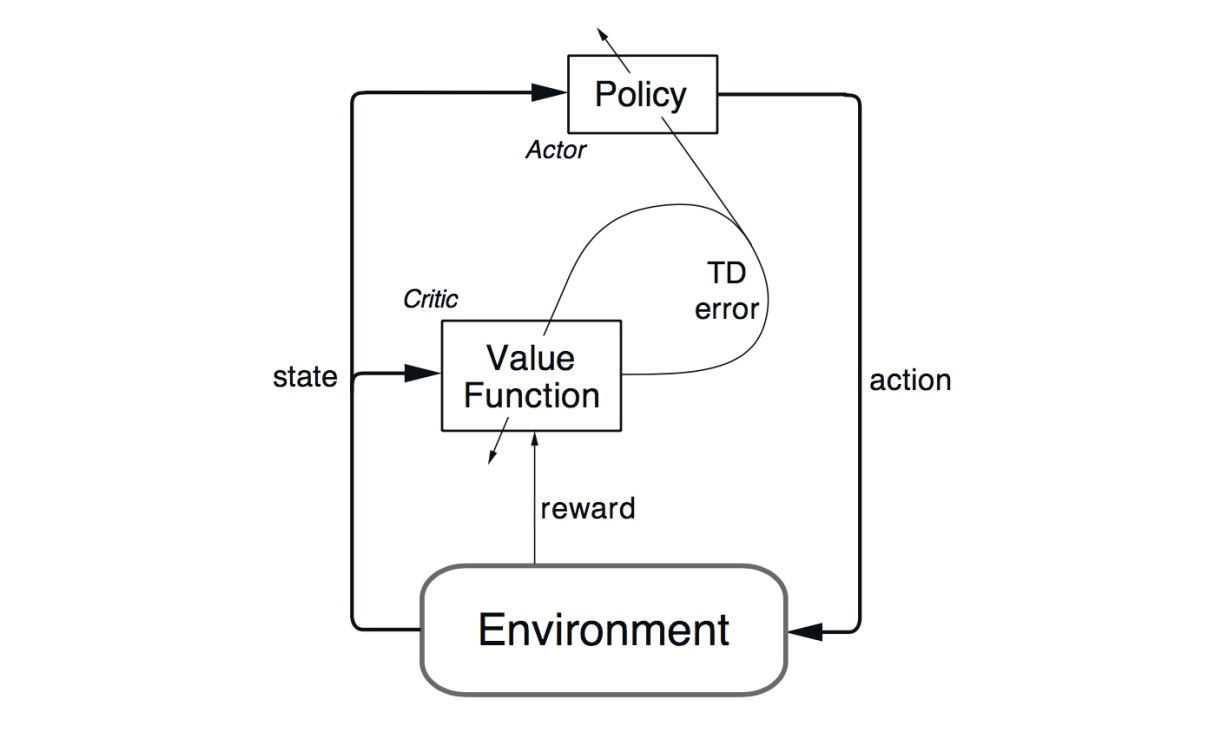
\includegraphics[width=\textwidth]{gfx/actor_critic_model}
	\caption{Actor Critic Model, Quelle: \cite{medium:actor_critic}}
	\label{fig:actor_critic_model}
\end{figure}

Actor-Critic ist eine Mischung beider Ansätze.
A2C steht für Advantage Actor Critic und gehört zu der Familie der Actor Critic Methoden.
Die grundlegende Idee dahinter ist das Aufteilen des Modells in zwei Teile: Einen Actor und einen Critic.
Der Actor nimmt die Policy-basierte Rolle ein.
Er berechnet zu einem bestimmten Zustand die zu wählende Aktion. Der Critic setzt den Value-basierten Ansatz um.
Er berechnet auf Grundlage der gewählten Aktion des Actors und dem daraus resultierenden Zustand einen Wert, der die Güte der vom Actor getroffenen Aktion bestimmt.
Der Actor handelt also und der Critic bewertet ihn dabei.
Diese Dynamik lässt sich durch folgende mathematische Formel definieren \cite{theaisummer:actor_critic}: 

\begin{eqnarray}
	\Delta _{ \theta } J(\theta) = \sum_{t=0}^{T-1} \Delta_{ \theta } log _{ \theta } \pi _{ \theta } (a_{t} | s_{t}) A(s_{t}, a_{t})
\end{eqnarray}

J($\theta$) ist die Zielfunktion, die es zu maximieren gilt und $\pi$ ist die Policy. Beide sind abhängig von $\theta$, den Gewichten des Neuronalen Netztes. Verändert sich $\theta$, dann verändert sich die Policy und dadurch auch das Ergebnis der Zielfunktion. Die Policy wir durch den Actor abgebildet und nimmt als Input einen Zustand s entgegen. Output des NNs ist eine stochastische Verteilung aller möglichen Aktionen. R ist der Reward, bzw. die Bewertung des Critics für die gewählte Aktion. Ziel ist es also mit möglichst hoher Wahrscheinlichkeit eine Aktion zu wählen, die den größtmöglichen Reward erbringt. Die Berechnungen können sowohl über einzelne, als auch mehrere steps erfolgen. Berechnungen über mehrere  steps sind allerdings stabiler und von der Berechnung her rentabler \cite{towardsdatascience:actor_critic}.

\begin{eqnarray}
	\Delta _{ \theta } J(\theta) = \sum_{t=0}^{T-1} \Delta_{ \theta } log _{ \theta } \pi _{ \theta } (a_{t} | s_{t}) A(s_{t}, a_{t})
\end{eqnarray}

In Abbildung 1 sind m die Episoden und T die steps, über die die Veränderung der Gewichte ermittelt wird.
Um das Modell stabiler gegenüber Veränderungen zu machen, ist es außerdem möglich ein Experience Replay einzuführen, wie im Kapitel \ref{sec:rl:dqn:experience_replay} beschrieben.


\subsubsection{Discounted Rewards}

Werden zur Berechnung von J($\theta$) mehrere Steps verwendet, so kann es dazu kommen, dass die Summe der Rewards aller Steps 0 ergibt. Das NN würde also nichts lernen. Dies kann durch Discounted Rewards verhindert werden. Die Idee hinter Discounted Rewards ist es, aufeinander folgende Steps mit einem Discount Faktor zu parametrisieren, sodass die Rewards zukünftiger Aktionen weniger Wert sind, als die Rewards unmittelbarer Aktionen. Gute Aktionen werden so auch nicht herausgezögert, um den Reward zu maximieren \cite{towardsdatascience:actor_critic}.

\begin{eqnarray}
	R_{t} = \sum_{t'=t}^{T} \gamma^{t'}r_{t'}
\end{eqnarray}

\subsubsection{Advantage Baseline}
Bei der Verwendung von Value-Functions ist es problematisch, dass die Werte eine sehr hohe Variabilität aufweisen. Um dem entgegen zu wirken und den Lernerfolg zu stabilisieren, kann man eine sogenannte Baseline verwenden. Von einer Baseline ausgehend wird die Abweichung zu dieser errechnet. Dieser Wert ist ab da an der Ergebniswert der Value-Function, der für das Update des NNs verwendet wird. Eine mögliche Baseline ist die Advantage-Baseline. Die Funktion A mit den Parametern Zustand s und Aktion a zum Zeitpunkt t zur Bestimmung des Advantage ist wie folgt definiert \cite{towardsdatascience:actor_critic}:

\begin{eqnarray}
	A(s_{t}, a_{t}) = Q(s_{t}, a_{t}) - V(s_{t})
\end{eqnarray}

Der Advantage ist also die Differenz zweier Value-Funktionen Q und V. Q ist hierbei der vom Critic berechnete Q-Value und V der im Durchschnitt zu erwartende Wert basierend auf dem momentanen Zustand. Um die Berechnung zweier unterschiedlicher Value-Funktionen zu vermeiden, wird über den sogenannten TD-Error der Advantage approximiert.

\begin{eqnarray}
	A(s_{t}, a_{t}) = r(t) + \gamma V(s_{t-1}) - V(s_{t})
\end{eqnarray}

r ist hierbei die Belohnung zum Zeitpunkt t und $\gamma$ die verwendete Discount Rate. Die Discount Rate bestimmt mit welchem Faktor der Wert alter Aktionen mit in den Advantage einfließen soll.


\subsection{PPO}
PPO steht f"ur Proximal Policy Optimization und folgt der Policy Gradient Methode. Im Jahr 2017 hat das Team von OpenAI diesen neuen Algorithmus
ver"offentlicht, mit dem Ziel, einen Reinforcement Algorithmus zu erstellen, der folgende drei Eigentschaften erf"ullt\cite{openai:ppo}:
\begin{itemize}
	\item \textbf{Easy Code:} Hinter dem Algorithmus verbirgt sich kein "uberm"aßig komplizierter Code
	\item \textbf{Sample Efficient:} Der Algorithmus zieht den maximalen Ertrag aus jedem einzelnen Datum
	\item \textbf{Easy To Tune:} Hinter dieser Methode verbergen sich weniger Hyperparameter als hinter anderen Reinforcement-Learning-Algorithmen
\end{itemize}
PPO ist ein on-line lernender Algorithmus, er lernt also nicht aus vergangenen Erfahrungen, die in einem Replay-Buffer gespeichert werden, sondern direkt aus den aktuellen Erfahrungen des aktiven Agenten.
Der Agent sammelt also Erfahrungen und sobald gen"ugend Daten vorhanden sind - man spricht von einem Batch - wird die Policy auf Grundlage dieser aktuellen Erfahrungen verbessert. Anschließend wird das soeben verwendete Batch von Daten gel"oscht, da es seinen Zweck erf"ullt hat.
\newline
Policy Gradient Methoden sind dadurch in der Regel weniger ``sample-efficient'', da sie jede Erfahrung des Agenten nur einmalig benutzen.

\subsubsection{Policy Gradient Methode}
Proximal Policy Optimization ist eine Policy Gradient Methode.
Im folgenden ist ein Policy Gradient Loss zu sehen.

\begin{eqnarray}
L^{PG}(\theta) = \hat{\mathbb{E}}_{t}[\:log\: \pi_{\theta}\:(a_{t}|s_{t})\:\hat{A}_{t}]
\end{eqnarray}

$\pi_{\theta}$ ist die aktuelle Policy, also der Output des Netzwerks, der vorgibt, welche Aktion als n"achstes gew"ahlt werden soll.
$\hat{A}_{t}$ ist die Advantage-Funktion. Sie versucht die relative G"ute der ausgew"ahlten Aktion einzusch"atzen und setzt sich aus den folgenden zwei Komponenten zusammen:

\begin{eqnarray}
\hat{A}_{t} = Discounted\: rewards - Baseline\: estimate
\end{eqnarray}

Die Discounted Rewards sind eine Gewichtung der rewards. Der Agent gewichtet diejenigen Aktionen mehr, die schneller einen Reward erzeugen.
Das Baseline Estimate ist eine Value Function. Sie versucht einzusch"atzen, wie hoch die Discounted Rewards in der Zukunft ab dem jetzigen Zeitpunkt ausfallen werden.

Das Advantage-Estimate l"ost also die Frage: War die Aktion, die ausgew"ahlt wurde besser oder schlechter als erwartet?
Ist $\hat{A}_{t}$ positiv (der Gradient ist also positiv), bedeutet dies, dass die ausgew"ahlte Aktion zu einem besseren Ergebnis gef"uhrt hat, als erwartet.
Als Folge dessen wird die Wahrscheinlichkeit, diese Aktion in der Zukunft erneut zu w"ahlen, erh"oht.
Wenn $\hat{A}_{t}$ negativ ist, wird die Wahrscheinlichkeit f"ur diese Aktion verringert.

\subsubsection{Trust Region Methode}
Ein Nachteil der Policy Gradient Methoden tritt auf, wenn man zu oft den Gradient Descend auf ein einzelnes Batch anwendet. Dann läuft die Optimierung der Policy sehr stark in eine Richtung, bis sie nicht mehr brauchbar ist. Beispielsweise kann die aktuelle Ver"anderung der Policy so schlecht gew"ahlt worden sein, dass dadurch im n"achsten Schritt gar kein gutes Ergebnis mehr erzielt werden kann, was letztendlich dazu f"uhrt, dass sich die Policy nie mehr positiv entwickeln kann, sondern immer schlechter wird.
\newline
Um diesem Problem entgegenzuwirken, wurde die Trust Region Methode erfunden. Ziel dieser Methode ist es, dass die Optimierung einer Policy niemals zu weit entfernt von der vorherigen Policy ist.
\subsubsection{Der Algorithmus}
Das ist die Grundidee der Proximal Policy Optimization.
Hierf"ur wurde ein neuer Parameter eingef"uhrt, der die Beziehung zwischen alter und neuer Policy beschreibt und somit sicherstellt, dass sich die neue Policy nicht weiter als gew"unscht von der alten Policy entfernt.
Dieser neue Parameter muss im Lernprozess mit ber"ucksichtigt werden, so dass der Aufwand erh"oht wird. Darum verwendet PPO diesen neuen Parameter direkt als eines der Optimierungsziele, er muss also nicht als externer Hyperparameter angegeben werden.
\newline
Im Allgemeinen funktioniert der PPO-Lernalgorithmus so wie ein Trust Region Policy Optimization Algorithmus. Es werden Policy Updates so durchgef"uhrt, dass die Schritte von einer aktuellen Policy zu einer neuen Policy klein gehalten werden.
Wenn eine Aktion positive Auswirkungen hat, wird die Wahrscheinlichkeit f"ur diese Aktion erh"oht, jedoch, wie zuvor beschrieben, nicht zu sehr.
Des Weiteren wird die Wahrscheinlichkeit f"ur diejenigen Aktionen verringert, die negativ f"ur das zu erreichende Ziel waren. Auch hier gilt wieder, dass die Verringerung der Wahrscheinlichkeit nicht zu stark gew"ahlt wird.
Wenn eine Aktion allerdings sehr negative Auswirkungen hat, der Algorithmus aber im letzten Schritt diese Aktion als sehr gut eingestuft hat, dann wirkt der PPO-Algorithmus dieser falschen Folgerung entgegen und verringert die Wahrscheinlichkeit, diese Aktion erneut zu w"ahlen, wieder stark.\cite{schuh:2017}



% ----------------------------------------------------------------------------------
% Kapitel: Praktische Umsetzung
% ----------------------------------------------------------------------------------
\section{Praktische Umsetzung}
\subsection{Programmiersprache}
Die Wahl der Programmiersprache ist bei einem neuen Projekt immer eine der ersten wichtigen Entscheidungen.
Im Bereich Machine Learning fällt diese Entscheidung jedoch relativ leicht.
Die Meistgenutzten Sprachen sind in diesem Fall \textit{Python}, \textit{C++}, \textit{JavaScript}, \textit{Java} und \textit{C\#}.
Die einzige Sprache, welche eine native ausführbare Datei ohne Interpreter kompilieren kann ist in diesem Fall C++.
Jedoch überzeugt die Masse an Bibliotheken und Machine Learning Projekten sowie die Einfachheit von Python.
Python ist keinesfalls eine schnelle Sprache, jedoch sind die meisten kritischen Funktionen nativ in C implementiert.
JavaScript ist sehr ähnlich zu Python und bietet gegenüber Python keine klaren Vorteile.
Java und C\# werden häufig für große Firmenprojekte eingesetzt \cite{github:blog:ml_langs}.
Diese sind zwar schneller in der Ausführung als Python, bieten jedoch viel weniger Bibliotheken.

Aus diesen Gründen wurde sich schließlich für Python entschieden.

\subsection{Framework}
Eines der Ziele des Projekts war die Erstellung eines Frameworks, welches das Training von beliebigen Agenten generalisieren und vereinfachen soll.
Damit ist es möglich innerhalb kürzester Zeit ein neues Spiel oder einen neuen Agenten hinzuzufügen.
Für das Generalisieren von Agenten wird die abstrakte Klasse \textit{IAgent} (Abb. \ref{fig:agentpy}) verwendet.
Diese impliziert, dass jeder Agent das Attribut \pyth{NAME} besitzen muss.
Der Name wird z.B. für die Darstellung in den Videos verwendet.

Die Methode \pyth{__init__} ist der Konstruktor der Klasse und bekommt eine Vielzahl an Parametern.
Dabei gibt \pyth{input_size} die Anzahl der zu beobachtenden Features bzw. die Auflösung des Bildes als Tupel in X- und Y-Richtung an.
Der Parameter \pyth{output_size} gibt die Anzahl an möglichen Ausgaben/Aktionen an, welche vom Agenten durchgeführt werden können.
Mit dem Parameter \pyth{training_mode} wird angegeben, ob der Agent trainieren oder die momentan geladenen Gewichte ausschließlich lesen soll.
Der Parameter \pyth{is_conv} gibt an, ob die Eingabe Pixeldaten sind und ein Faltungsnetzwerk genutzt werden soll oder nicht.
Über den Parameter \pyth{load_filename} wird der Dateipfad zu einer .mdl Datei angegeben, falls diese geladen werden soll.
Ist dieser \pyth{None}, wird kein Modell geladen.
Der Parameter \pyth{seed} ist eine Zahl, welche den Zufallsgenerator auf eine feste und bestimmte Sequenz von Zahlen festlegt.

Die Methode \pyth{save_model} wird zum speichern aller Gewichte und Agentkonfigurationen verwendet.
Einziger Parameter ist der Dateiname, unter dem das Modell zu speichern ist.

Die Methode \pyth{copy_from} kopiert die Gewichte einer anderen Instanz des gleichen Agenten.
Dies ist z.B. sinvoll, wenn ein Agent gegen sich selbst spielen soll, jedoch aus Effizienzgründen nur ein Agent trainiert wird.
Der einzige Parameter ist das Objekt des Agenten, von dem kopiert werden soll.

Die Methode \pyth{get_action} liefert für einen bestimmten Zustand eine Aktion für das Spiel zurück.
Einziger Parameter ist der momentane Zustand des Spiels, z.B. ein Bild in Form von Pixeldaten oder Spielerpositionen in Form eines Vektors.

Die Methode \pyth{update} trainiert den Agenten und liefert die dazu benötigten Informationen als Parameter.
Der erste Parameter \pyth{state} ist der Zustand des Spiels, bevor die letzte Aktion durchgeführt wurde.
Der zweite Parameter \pyth{action} gibt die Aktion an, welche vom Agenten ausgewählt wurde.
Der \pyth{reward} ist eine Zahl, welche die durchgeführte Aktion bewertet.
Der Parameter \pyth{next_state} ist der resultierende Zustand nach Ausführung der Aktion und \pyth{done} gibt an, ob dies das Ende einer Runde des Spiels war.

\begin{figure}[!h]
\begin{python}
class IAgent(metaclass=ABCMeta):
	@property
	@abstractmethod
	def NAME(self)

	@abstractmethod
	def __init__(self, input_size, output_size, training_mode, is_conv, load_filename, seed)

	@abstractmethod
	def save_model(self, filename)

	@abstractmethod
	def copy_from(self, model)

	@abstractmethod
	def get_action(self, state)

	@abstractmethod
	def update(self, state, action, reward, next_state, done)
\end{python}
\caption{Abstrakte Klasse IAgent, \textit{agents/agent.py}}
\label{fig:agentpy}
\end{figure}

\subsubsection{Gym}
\label{sec:pract:framework:gym}
Sehr viele Open Source Projekte verwenden das \textit{Gym} Framework von \textit{OpenAI}.
Dieses legt fest, welche Methoden und Attribute ein sogenanntes \textit{Environment} besitzen muss.
Ein Environment ist die Umgebung, in der der Agent eine Aktion durchführen kann und diese Aktion eine Auswirkung haben kann.
Spiele wie Pong werden als ein solches Environment angeboten.

Der Environment-Lifecycle besteht aus 2 Teilnehmern: Dem Agenten und dem Environment selbst (Abb. \ref{fig:pract:framework:gymenv}).
Als erstes wird das Environment erstellt und initialisiert.
Dabei entsteht die erste \textit{Observation}.
Der Agent verwendet die Observation, um zu entscheiden welche Aktion ausgeführt werden soll und führt die neue Aktion auf dem Environment aus.
Eine Observation beinhaltet alle relevanten Informationen für den Agenten.
Diese können auf verschiedene Arten gespeichert werden.
Für Pong könnte man z.B. die Position und Geschwindigkeit beider Paddles und des Balls angeben.
In der Realität hat man aber leider oft keine genauen Daten bzw. ist genau das Extrahieren dieser Daten das Problem, welches gelöst werden soll.
In diesem Fall verwendet man meistens Bilder für die Observations.

\begin{figure}[!h]
	\centering
	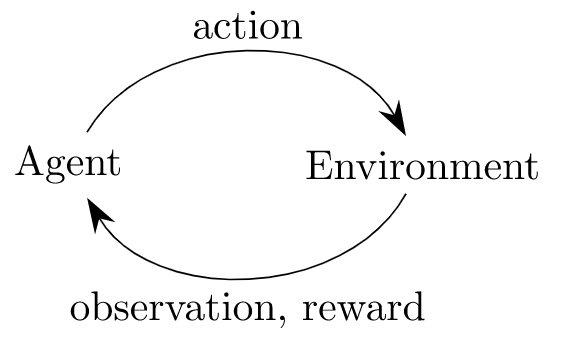
\includegraphics[width=0.3\textwidth]{gfx/gym_env}
	\caption{Gym Environment-Lifecycle, Quelle: \cite{gym:doc:env}}
	\label{fig:pract:framework:gymenv}
\end{figure}

Im groben gibt es 5 wichtige Methoden, welche für ein Gym-Environment implementiert werden müssen.
Die Methode \pyth{make} erstellt ein neues Environment und erhält den Namen als einzigen Parameter.
Die Methode \pyth{reset} setzt ein Environment zurück und wird auch zum Initialisieren verwendet.
Die Methode \pyth{step} führt einen Schritt in dem Environment aus. Parameter ist die durchzuführende Aktion.
Rückgabewert ist eine Observation und der Reward für die durchgeführte Aktion.
Der Reward ist eine reelle Zahl und gibt an, wie gut oder schlecht eine ausgeführte Aktion war.
Die Methode \pyth{render} zeichnet das Environment auf den Bildschirm und lässt den Anwender beobachten, was gerade passiert.
Die Bildrate wird in diesem Falle jedoch meistens auf 30 oder 60 Bilder pro Sekunde festgelegt und verlangsamt das Training.
Die Methode kann ein Bild des Environments zurückgeben, welches statt der Observation verwendet werden kann.
Zu guter Letzt gibt es die Methode \pyth{close}, welche das Environment schließt und den Speicher freigibt.

\subsubsection{Environment-Wrapper}
Da es verschiedene Arten von Environments gibt und alle für das Training ein wenig angepasst werden müssen, wurde der \textit{Environment-Wrapper} implementiert.
Dieser wirkt nach außen wie ein ganz gewöhnliches Gym-Environment, kann jedoch intern für jedes Environment zuvor angepasste Änderungen vornehmen.
Der Wrapper hat 3 Aufgaben:
\begin{itemize}
	\item Support für Gym-Environments und Spiele in anderem Format
	\item Angepasstes Pre-Processing
	\item Erstellen von Videoaufnahmen
\end{itemize}

Es wird großen Wert auf Support von vielen verschiedenen Spielen gelegt.
Daher kann der Wrapper jedes Spiel in eine Gym-Environment-Form pressen.

Eine weitere sehr wichtige Funktion ist das Pre-Processing von Observations - in diesem Fall speziell auf Bilddaten ausgelegt.
Da die Environments sehr unterschiedlich sind, müssen die Bilddaten für besseres Training vereinfacht werden.
Ein Agent lernt sehr viel schneller, wenn nur die wichtigen Spielelemente auf den Bildern vorhanden sind und alles unwichtige ausgeblendet wird.
Dafür unterstützt der Wrapper 3 generische Funktionen, mithilfe derer die Bilder in die gewünschte Form transformiert werden können.
Diese Funktionen sind: \textbf{Cropping}, \textbf{Resizing} und \textbf{Recoloring}.

Beim \textbf{Cropping} kann ein Bereich festgelegt werden, welcher aus dem original Bild ausgeschnitten und weiter verwendet werden soll.
Somit kann man unwichtige oder gar störende Stellen wie z.B. den Punktestand bei Pong oder den Boden bei Flappybird entfernen.

Das \textbf{Resizing} kann das Bild auf eine neue Größe skalieren, wobei das Seitenverhältnis nicht gleich bleiben muss.
Es gibt sehr viele verschiedene Methoden um ein Bild zu skalieren, jedoch gehen bei allen Methoden verschiedene Bilddaten verloren.
Man sollte im Vorraus immer eine geeignte Größe ausrechnen, damit z.B. wichtige Umrandungen oder sehr kleine Objekte nicht einfach verschwinden.
Die Bilder sollten im allgemeinen nicht zu groß sein, da sonst das Training stark verlangsamt wird.

Das \textbf{Recoloring} ist ein wichtiger Schritt, welcher einen bestimmten Farbbereich suchen und ersetzen kann.
Als aller erstes wird das Bild in Graustufen konvertiert.
Somit werden jetzt statt 3 Bytes pro Pixel nur noch 1 Byte verwendet, was das Training ungemein erleichtert.
Jetzt können Farben in einem bestimmten Bereich wie z.B. 0-30 (sehr dunkle Farbtöne) mit dem Wert 0 ersetzt werden.
Alle anderen Pixel (31 - 255: helle bis sehr helle Farbtöne) werden mit einer 1 ersetzt.
Jetzt ist das Bild binärisiert bzw. fertig bearbeitet und kann vom Agenten zum Training genutzt werden.

Eine weitere wichtige Funktion des Wrappers ist der \textbf{Frame-Stack}.
Mit einem einzelnen Bild kann man kaum eine Aussage über Geschwindigkeit oder gar nur eine Richtung der Bewegung eines Objektes treffen.
Der Frame-Stack hat eine maximale Kapazität (Standard ist 4) und speichert die letzten Bilder und das neuste Bild.
Alle Bilder werden nach dem Pre-Processing gespeichert.
Jedes Bild kommt in einen seperaten Channel des Tensors.
Das Ergebnis all dieser Transformationen kann auf Abb. \ref{fig:pract:framework:wrapper:pong} und Abb. \ref{fig:pract:framework:wrapper:flappy} beobachtet werden.

\begin{figure}[!h]
	\centering
	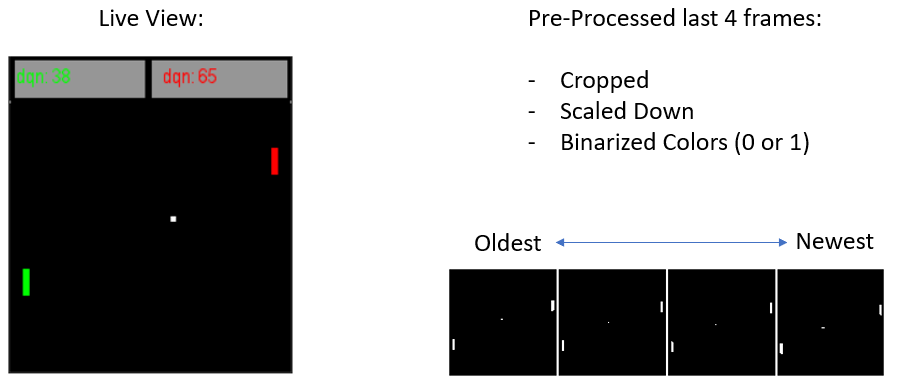
\includegraphics[width=0.8\textwidth]{gfx/pp_pong}
	\caption{Pre-Processing: Pong, Quelle: Eigene Darstellung}
	\label{fig:pract:framework:wrapper:pong}
\end{figure}

\begin{figure}[!h]
	\vspace{3cm}
	
	\centering
	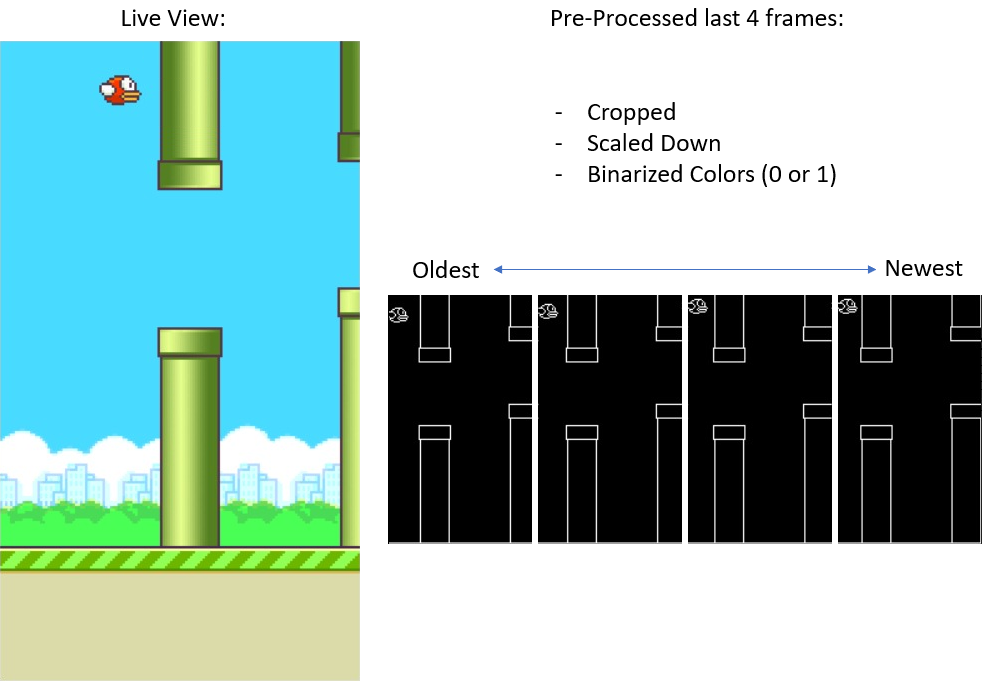
\includegraphics[width=0.9\textwidth]{gfx/pp_flappy}
	\caption{Pre-Processing: Flappybird, Quelle: Eigene Darstellung}
	\label{fig:pract:framework:wrapper:flappy}
\end{figure}

\newpage

\subsubsection{PyTorch}
Python bietet viele Machine Learning Frameworks.
Darunter sind \textit{Keras}, \textit{PyTorch} und \textit{TensorFlow}.
Alle drei genannten Frameworks sind Open Source, aber unterscheiden sich deutlich in der Handhabung und Geschwindigkeit \cite{edureka:ml_frameworks}.
Keras ist ein high-level Wrapper für schon bestehende low-level Frameworks wie TensorFlow oder PyTorch (nicht in Keras implementiert).
Keras ist sehr leicht zu benutzen und versteckt sehr viele Details der Implementierung der Netze.
Daher ist Keras für unsere Anwendung eher nicht geeignet, da das Ziel der Aufbau von fundamentellem Wissen über Reinforcement Learning und Machine Learning (speziell Deep Neural Networks) ist.
Bei der Geschwindigkeit liegen PyTorch und TensorFlow sehr nah zusammen, wobei TensorFlow meistens ein klein wenig schneller ist.
Jedoch ist PyTorch viel leichter zu benutzen und zu debuggen als TensorFlow \cite{edureka:ml_frameworks}.
Somit wurde sich letztendlich für PyTorch entschieden.


\subsubsection{Automatisierte Hyperparametersuche}
Für Offline-Machine-Learning Verfahren gibt es bereits etablierte Bibliotheken wie scikit-learn, die eine automatisierte Suche von Hyperparametern erlauben.
Reinforcement Learning wird allerdings zum Zeitpunkt der Durchführung des Projektes nicht von der Bibliothek unterstützt und unser Team fand auch keine anderen Bibliotheken, mit denen sich eine automatierte Hyperparametersuche realisieren ließ.
\newline
Deswegen wurde diese Funktionalität im Zuge des Projektes selbst programmiert.
Unter Ausführung eines Scriptes lässt sich die beste Kombination innerhalb einer zuvor definierten Menge an Parameterkombinationen ermitteln.
Kombinationen und durchzuführender Konsolenbefehl zur Bestimmung von Agententyp und anderen Umgebungsparametern werden in einer JSON -Datei festgelegt.
Im Falle zuvor definierter Parameter spricht man von einer GridSearch. \cite{medium:gridsearch}
\newline
Das Programm wird mit allen im Vorfeld spezifizierten Kombinationen nacheinander gestartet wird.
Die Ergebnisse werden gesammelt in einem Ordner gespeichert und können während und nach Durchführung der Suche eingesehen werden.


\subsection{Verwendete Spiele}
Die zu trainierenden Spiele wurden aufgrund von unterschiedlichen Faktoren gewählt.
Um zu Beginn die verschiedenen Agenten zu testen, wurden leichte Probleme wie \textit{CartPole} und \textit{LunarLander} verwendet.
Diese sind Standardprobleme aus dem Reinforcement Learning und eignen sich bestens zur Überprüfung der allgemeinen Performance der Agenten.
Nachdem die Standardprobleme mit gutem Erfolg trainiert waren, konnten nun die Faltungsnetzwerke zur Bilderkennung implementiert werden.
Dazu wurden zwei neue Spiele gewählt: \textit{Pong} und \textit{Flappy Bird}.
Die Agenten trainieren diese Spiele ausschließlich über die Bilddaten.
Diese Spiele wurden gewählt, da sie eine gewisse Komplexität aufweisen, aber nicht viel zu komplex für das Training sind (wie z.B. Super Mario).

\subsubsection{Cart Pole}
Bei Cart Pole handelt es sich um das Standardproblem des Reinforcement Learnings.
Ein kurzer Stab, dessen oberes Ende frei in der Luft steht und dessen unteres Ende beschient auf einer Oberfläche befestigt ist, soll durch horizontale Bewegungen in Balance bleiben (Abb. \ref{fig:pract:cartpole}).
Um die Balance aufrecht zu halten und den Stab vor dem Kippen zu bewahren, muss zu jedem Zeitschritt entweder nach rechts (+1) oder links (-1) ausbalanciert werden. 
Bewertet wird, wie lange der Stab balanciert gehalten werden kann.
Pro Zeitschritt (step) innerhalb einer Episode gibt es einen Punkt.
Als gescheitert gilt die Episode ab einer Neigung von 12 Grad oder sobald der sich der Stab um mehr als 2,4 Einheiten vom Startpunkt entfernt hat.
Ab einer durchschnittlichen Belohnung von 195 bei einer Episodenlänge von 200 Schritten zählt dieses Problem als gelöst.
Das Environment bekommt die Observations direkt als Array, welches die Cart Position, Geschwindigkeit und Pole Geschwindigkeit enthält.

\begin{figure}[!h]
	\centering
	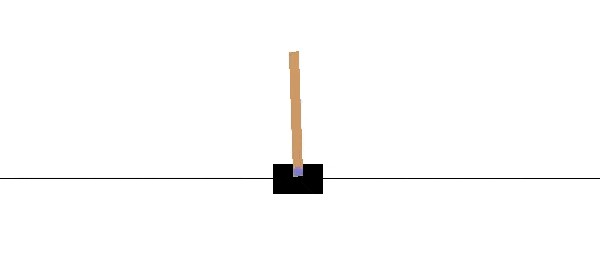
\includegraphics[width=0.6\textwidth]{gfx/cartpole}
	\caption{Aufnahme: CartPole, Quelle: Eigene Darstellung}
	\label{fig:pract:cartpole}
\end{figure}

Dieses Problem wurde von allen Agenten gelöst.
Das DQN (Abb. \ref{fig:pract:cartpole:dqn}) braucht zwar mehr Episoden als das A2C (Abb. \ref{fig:pract:cartpole:a2c}), lernt dafür mehr Episoden pro Zeit und kommt daher auf ungefähr die gleiche Trainingsdauer.

\begin{figure}[!h]
	\centering
	\begin{minipage}{.5\textwidth}
		\centering
		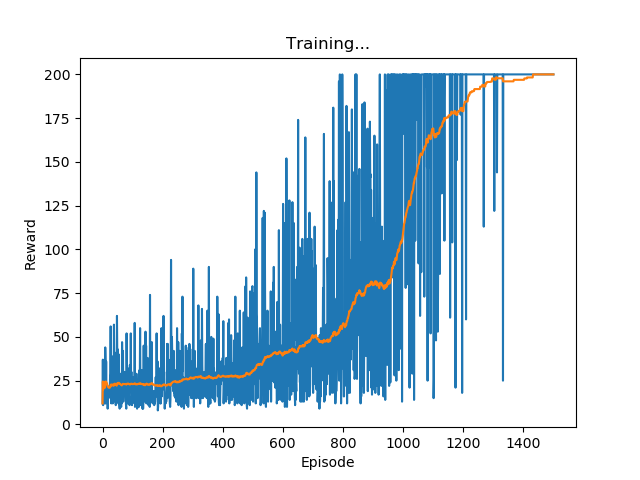
\includegraphics[width=0.9\textwidth]{gfx/dqn_cartpole_model_1500}
		\caption{DQN CartPole Training}
		\label{fig:pract:cartpole:dqn}
	\end{minipage}%
	\begin{minipage}{.5\textwidth}
		\centering
		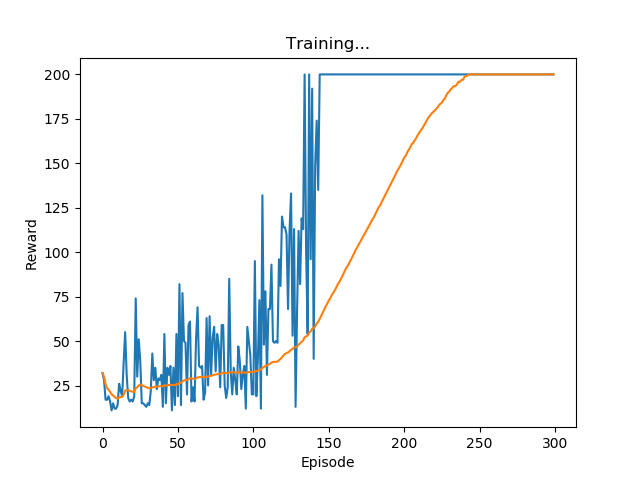
\includegraphics[width=0.9\textwidth]{gfx/model_300}
		\caption{A2C CartPole Training}
		\label{fig:pract:cartpole:a2c}
	\end{minipage}
\end{figure}

\newpage

\subsubsection{Lunar Lander}
Lunar Lander ist ein weiteres klassisches Problem aus dem Reinforcement Learning.
Der Agent muss bei diesem Environment ein Raumschiff zwischen zwei Flaggen landen, welche sich immer in der Mitte (0, 0) der Karte befinden (Abb. \ref{fig:pract:lunar}).
Die Eingabe ist komplexer und besteht aus 4 möglichen Aktionen: Nichts tun, linkes Triebwerk zünden, rechtes Triebwerk zünden und Haupttriebwerk zünden.
Auch die Bewertung ist bei diesem Problem komplexer gestaltet.
100 -- 140 Punkte gibt es dafür, dass das Raumschiff sich vom oberen Bildschirmrand auf den Boden bewegt und die Geschwindigkeit vor dem Landen abbremst (gemessen wird nur die Y-Achse).
Jedes der zwei Beine gibt bei Bodenkontakt weitere +10 Punkte.
Die Benutzung des Haupttriebwerks gibt pro Frame -0,3 Punkte, damit das Raumschiff nicht wieder nach oben fliegt oder zu lange in der Luft bleibt.
Eine Begrenzung für Treibstoff gibt es jedoch nicht.
Landet das Raumschiff zwischen den zwei Flaggen, gibt es weitere +100 Punkte, stürzt es jedoch ab (Geschwindigkeit bei Bodenkontakt zu hoch) gibt es 100 Punkte abzug.
Das Environment bekommt die Observations direkt als Array, welches die Position, Geschwindigkeit und Winkel des Raumschiffes, sowie den Bodenkontakt zu den Beinen als Boolean enthält.

Dieses Problem konnte nur vom DQN (Abb. \ref{fig:pract:lunar:dqn}) mit befriedigender Leistung trainiert werden. 

\begin{figure}[!h]
	\centering
	\begin{minipage}{.5\textwidth}
		\centering
		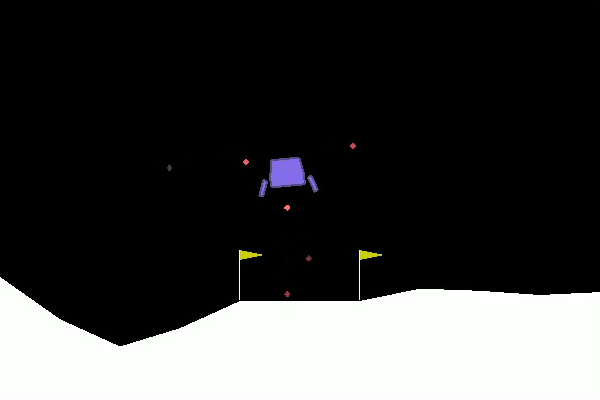
\includegraphics[width=0.9\textwidth]{gfx/LunarLander}
		\caption{Aufnahme: LunarLander}
		Quelle: Eigene Darstellung
		\label{fig:pract:lunar}
	\end{minipage}%
	\begin{minipage}{.5\textwidth}
		\centering
		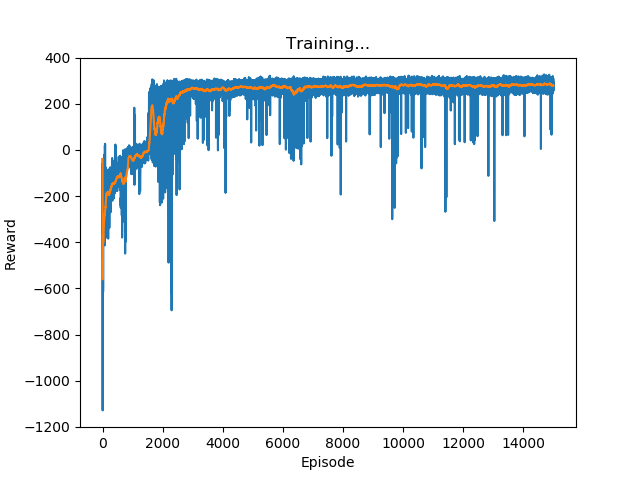
\includegraphics[width=0.9\textwidth]{gfx/dqn_lunarlander_model_15000}
		\caption{DQN LunarLander Training}
		\label{fig:pract:lunar:dqn}
	\end{minipage}
\end{figure}

\newpage

\subsubsection{Custom Pong}
Dieses Environment ist eine Adaption des bekannten Atari Klassikers Pong von Karol Arndt und Oliver Struckmeier an der Aalto Universität.
Ziel des Spiels ist es, den Ball mithilfe des Paddles in das gegnerische Tor zu stoßen, ohne dabei selbst ein Tor zu kassieren (Abb. \ref{fig:pract:framework:wrapper:pong}).
Die Eingabe besteht aus 3 möglichen Aktionen: Nach oben bewegen, nach unten bewegen und stehen bleiben.
Die initiale Bewertung ist relativ simpel, wobei ein Tor für den Gegner einen negativen Punkt und ein eigenes Tor einen positiven Punkt gibt.
Aus Testzwecken wurde diese Bewertung ein wenig verbessert, indem auch der vertiakle Abstand des eigenen Paddles zum Ball bei einem Punkt für den Gegner mitbeachtet wird.
Je größer dieser ist, desto mehr negative Punkte gibt es.
Dies sollte das Training verschnellern und zu besseren Ergebnissen führen, jedoch hatte es kaum Auswirkungen und in manchen Fällen wurde das Training sogar langsamer.
Daraus folgt, dass simplere Bewertungen meistens auch leichter zu lernen sind.
Die Observations bei diesem Environment sind die Pixeldaten der einzelnen Bilder.

Da es bei Pong 2 Spieler gibt, ist es in dieser Version auch möglich die Gegner-KI auszuwählen.
Zur Auswahl stehen hier die \textit{SimpleAI} (welche das Paddle einfach immer auf Ballhöhe zu halten versucht), alle Agenten mit trainierten Modellen und eine Benutzergesteuerte Eingabe.

Gute Ergebnisse hat bei diesem Environment nur das DQN (Abb. \ref{fig:pract:pong:dqn_vs_simple}) erreicht.
Um den Agenten noch weiter zu verbessern, trainierte dieser gegen sich selbst (Abb. \ref{fig:pract:pong:dqn_vs_dqn}).
Das Ziel hierbei ist es nicht, den Reward weiter zu steigern, sondern die Episodendauer zu erhöhen.
Dabei hat nur einer der Agenten sein neuronales Netz trainiert und alle 1000 steps die Daten des Netzwerks mit dem anderen Agenten synchronisiert.
Das Ergebnis war eine sehr kompetitive Pong KI.

\begin{figure}[!h]
	\centering
	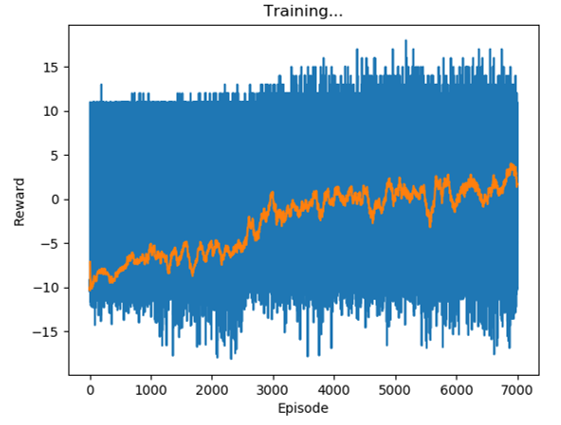
\includegraphics[width=0.6\textwidth]{gfx/dqn_custompong_model_7000}
	\caption{DQN vs SimpleAI CustomPong Training}
	\label{fig:pract:pong:dqn_vs_simple}
\end{figure}

\begin{figure}[!h]
	\centering
	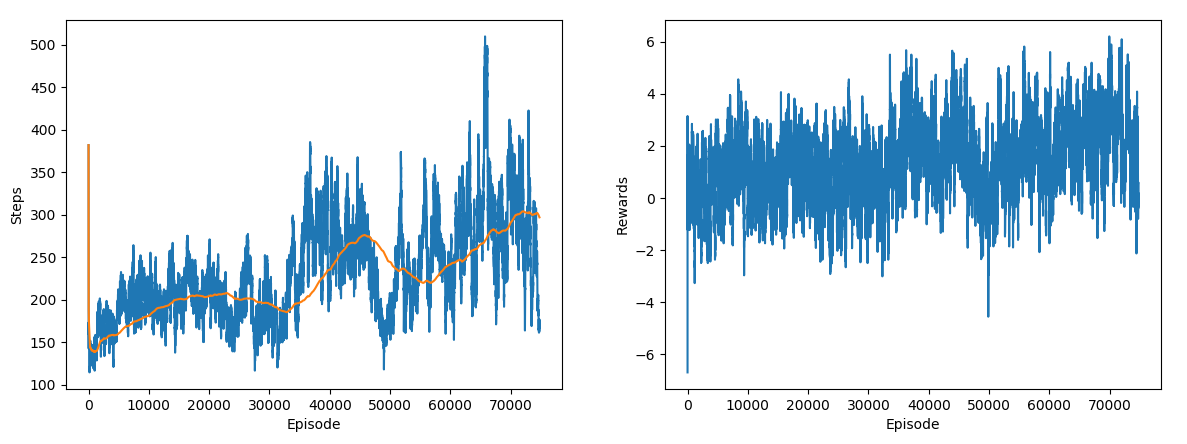
\includegraphics[width=1\textwidth]{gfx/dqn_custompong_model_70000}
	\caption{DQN vs DQN CustomPong Training}
	\label{fig:pract:pong:dqn_vs_dqn}
\end{figure}

\newpage

\subsubsection{Flappy Bird}
Flappy Bird ist ein sehr bekanntes Spiel für Smartphones.
Ziel ist es, einen nach rechts fliegenden Vogel an den vertikalen Säulen vorbei zu navigieren, ohne eine solche Säule zu berühren (Abb. \ref{fig:pract:framework:wrapper:flappy}).
Der Vogel wird durch die Schwerkraft automatisch nach unten gelenkt und jedes Tippen auf den Bildschirm lässt ihn einmal mit den Flügeln schlagen, womit er wieder ein Stück nach oben fliegt.
Die Bewertung ist relativ simpel gestaltet.
Jedes passierte Säulen-Paar gibt einen Punkt, das Treffen einer Säule gibt -5 Punkte.
Gestartet wird bei 0 Punkten.
Die Observations bei diesem Environment sind die Pixeldaten der einzelnen Bilder.

Befriedigende Ergebnisse hat bei diesem Environment nur das DQN (Abb. \ref{fig:pract:flappy:dqn}) erreicht.

\begin{figure}[!h]
	\centering
	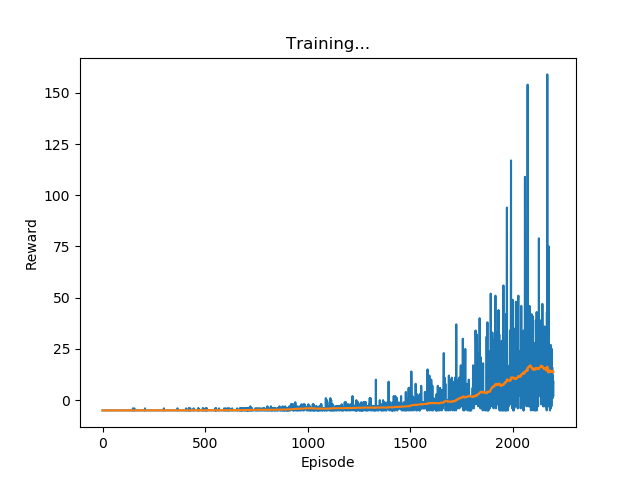
\includegraphics[width=0.6\textwidth]{gfx/dqn_flappybird_model_2200}
	\caption{DQN FlappyBird Training}
	\label{fig:pract:flappy:dqn}
\end{figure}

\newpage

% ----------------------------------------------------------------------------------
% Kapitel: Fazit
% ----------------------------------------------------------------------------------
\section{Fazit}
Jedes vorgestellte Environment konnte von mindestens einem Agenten gelöst werden.
Dabei waren die Ergebnisse fast immer besser, als die von menschlichen Spielern.
Dies verdeutlicht sehr, was für einen weiten Weg Machine Learning in den letzten Jahren zurückgelegt hast.

Jedoch bedeutet ein gutes Ergebnis nicht, dass sich die Anwendung für jedes Problem lohnt.
Wichtig ist bei Machine Learning immer, dass die Trainingsdaten von einer guten Quelle stammen.
Das Pre-Processing wirkt sich sehr stark auf den Lernerfolg aus und sollte immer mit Bedacht implementiert bzw. konfiguriert werden.
Kleinste Änderungen wie z.B. die Größe der Skalierung kann die Bilddaten nutzlos machen, da wichtige Informationen durch das Skalieren verloren gegangen sind.
Weiterhin ist es wichtig, den Reward nicht zu komplex zu wählen.
Ein komplexerer Reward führte fast immer zu einem ähnlichen Ergebnis aber erhöhte die benötige Zeit für das Training.
Weitere Probleme entstanden bei der Nutzung der Frameworks wie \textit{PyGame} oder \textit{PyTorch}.
Das Erstellen eines zweiten Fensters mit PyGame lässt Python auf Windows ohne weitere Exception einfach abstürzen.
Weiterhin gibt es in PyTorch auf Linux ein Memory Leak bei den Tensoren, welches trotz aller Anstrengungen nicht genau ausfindig gemacht werden konnte.
Das Training der Netze war gerade am Anfang sehr frustrierend, da man nicht genau weiß, ob das Problem die Hyperparameter sind, oder der Agent selbst.
Jedoch haben sich die Ergebnisse mit Verbesserungen am Agenten fast immer in auch in allen Environments verbessert, wodurch das Training sehr viel stabiler wurde und gegen Ende kaum noch ein Problem darstellte.
Vielmehr verlagerte man ab einem bestimmten Punkt das Augenmerk auf die grundsätzliche Trainingsgeschwindigkeit bzw. Trainingsdauer und versuchte, das \textbf{beste} (und nicht nur irgendein) Ergebnis zu erreichen.

Im Großen und Ganzen war das Projekt ein voller Erfolg und eine spannende Herausforderung. Alle Teilnehmer konnten einen tiefen Einblick in das Thema Reinforcement Leanring erlangen, so wie das wissenschaftliche Arbeiten beim Schreiben des Projektberichts vertiefen. Die Kommunikation innerhalb des Teams war sehr offen und stets konstruktiv.
Insgesamt hat sich der von Teammitglied Julian Dietrich entwickelte DQN-Agent als der M"achtigste herausgestellt. Die anderen Ans"atze A2C und PPO haben auch Potential gezeigt, lieferten in den hier getesteten Spielen aber nicht ganz so gute Ergebnisse wie der DQN-Agent.
Alle erprobten Ans"atze haben aber unterstrichen, dass es sich bei Reinforcement Learning um eine m"achtige und zukunftstr"achtige Disziplin des Machine Learning handelt. Hier ist noch lange nicht das Ende der Fahnenstange erreicht und mit einem weiteren Fortschritt - sei es durch effizientere Trainingsm"oglichkeiten mit leistungsst"arkerer Hardware oder durch neue, bessere Algorithmen - kann gerechnet werden.


\newpage

\section{Quellenverzeichnis}
\bibliographystyle{IEEEtran}
\bibliography{refs}

\end{document}
